%% -----------------------------------------------------------------------------

Trails and their properties give us the tools for a rigorous examination
of blame for Natural, Transient and Erasure Typed Racket in the setting of the 
mutants from section~\ref{sec:mutate}. In line with the discussion so far, 
our experimental process collects data to answer three initial questions
for our interesting debugging scenarios:
\begin{itemize}
\item[$Q_1$] Is blame useful in the context of Natural?

\item[$Q_2$] Is first blame useful in the context of Transient?

\item[$Q_3$] Is last blame useful in the context of Transient?

\end{itemize}

Furthermore, our experiment can compare the relative usefulness of blame
between any two of the three semantics. 
\begin{itemize}
\item[$Q_*$] Is blame for X more useful than blame for Y? (Where X and Y are any of Natural, Transient, or Erasure)
\end{itemize}


Table~\ref{fig:experiment-outline} summarizes how each question relates to
different kinds of trails/modes of the rational programmer. For example, experimental
question $Q_1$ asks whether blame is valuable for Natural and our experiment
uses the Natural blame and exception trails to answer it.

\begin{figure}[ht]
\center
{\begin{tabular}{l|c|c|c}
%% ---------------------------------------------------------------------------------------------------------------
                        & {\bf Natural}  & {\bf Transient} &  {\bf Erasure} \\ \hline 
%% ---------------------------------------------------------------------------------------------------------------
{\bf Blame}             &  $Q_1/Q_*$    &                  &                \\
{\bf First blame}       &               &     $Q_2/Q_*$    &                 \\
{\bf Last blame}        &               &     $Q_3/Q_*$    &                 \\
{\bf Exceptions}        &      $Q_1$    &     $Q_2/Q_3$    &      $Q_*$      \\
\end{tabular}}
  \caption{ Experimental questions and rational programmer modes.}
  \label{fig:experiment-outline}
\end{figure}

%% -----------------------------------------------------------------------------

In detail we answer $Q_1$  by comparing the success of the 
Natural blame and Natural exception trails for all interesting 
debugging scenarios from section~\ref{sec:mutate}.
  The first step is to construct each
mutant's scenario lattice and identify their interesting debugging
scenarios.
Our test
bed extends the trails that start from such roots according to the Natural-blame programmer.  If no scenarios
can be added to the trail, we check if
the last scenario of the trail type-checks or not. If it does, we record that the Natural-blame
trail is successful, and otherwise that it fails. We repeat the process for the
same roots again but for the other mode, Natural exceptions.
 Figure~\ref{fig:process}
summarizes this
experimental process for one mode of the rational programmer and connects
it with the mutations from section~\ref{sec:mutate}.
After completing the experiment, we calculate the
success/failure results of the trails to determine for each root whether Natural blame
is more useful than Natural exceptions. We
obtain a positive answer for
$Q_1$ when a root exists where the above is true since it is evidence that
there is at least one interesting scenario that the rational programmer
manages to debug because of blame. 
The process is analogous for $Q_2$ and $Q_3$, employing the respective
modes of the rational programmer.

For $Q_*$, the process is a bit more
involved. At a first level we proceed in a similar
manner except that we use two modes 
of the rational programmer from different semantics.
However, answering this question requires us to compare the percentage of scenarios
where one mode is more useful than the other and the inverse.
For instance, to
decide whether blame for Natural is more useful than first blame for Transient, 
we compare the percentage of interesting scenarios where 
Natural blame is more successful than Transient first blame 
with the percentage of interesting scenarios where Transient first blame 
is more successful than Natural blame. 
Finally we repeat these steps one more time to compare Natural blame and Transient last blame
and get a complete picture of the comparative usefulness of blame
in the two semantics.

\begin{figure}
  \centering
  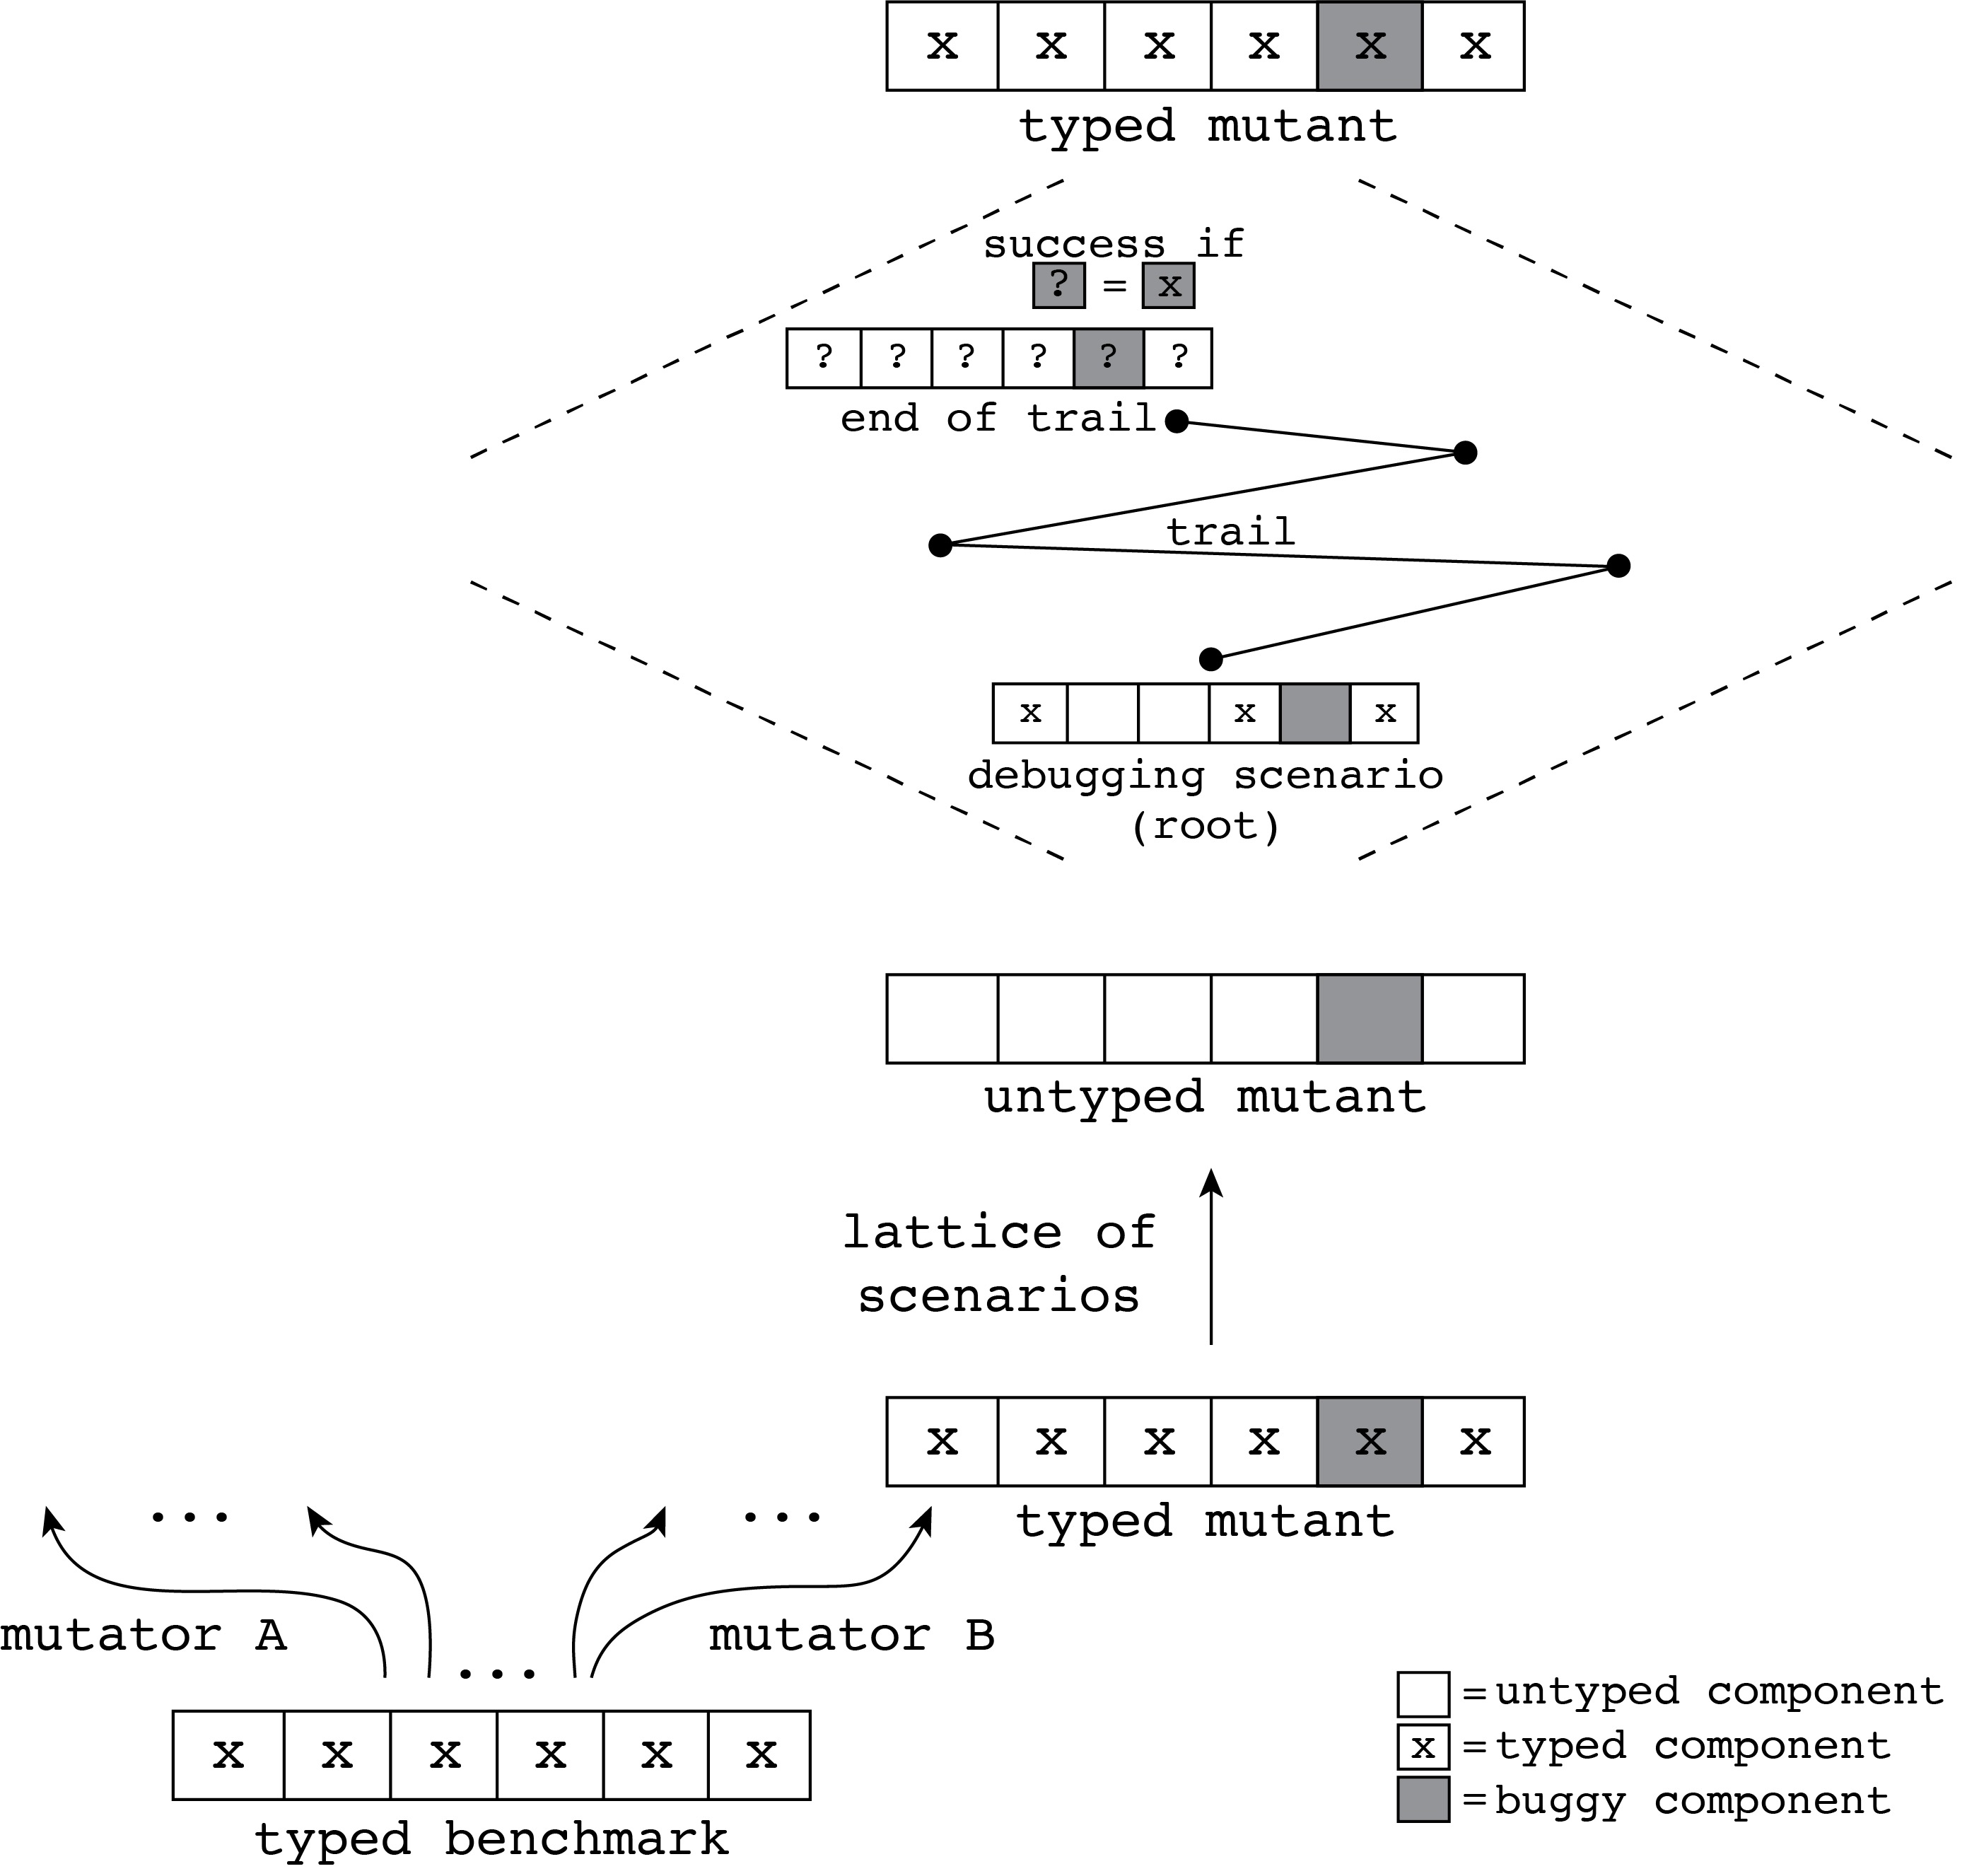
\includegraphics[scale=0.36]{./Images/process}
  \caption{The experimental process for one mode of the rational
  programmer}
  \label{fig:process}
\end{figure}

